\documentclass[12pt, a4paper]{article}
\usepackage[a4paper, bindingoffset=0.2in, %
left=0.5in,right=0.5in,top=0.5in,bottom=0.5in,%
footskip=.25in]{geometry}
\usepackage{graphicx}
\usepackage{amssymb}
\usepackage{amsmath}
\usepackage{hyperref}
\usepackage{physics}

\title{PSet8 Report}
\author{Ali Abolhassanzadeh Mahani}


\begin{document}
	\maketitle
	\section{First Order Differential Equation}
	The equation we are to solve is
	\begin{equation}
		R \dv{Q}{t} + \frac{Q}{C} = V
	\end{equation}
	for the values $V= 10 volts$, $R = 3000 \Omega$, $C = 1 \mu F$ and the simulation time from zero to $t = 0.5\, ms$.\\
	Since the numbers are a little overwhelming, we make parameter changes to come up with better numbers for our simulation.
	
	The change of variables is as follows:
	\begin{equation}
		\begin{aligned}
			&x \equiv \frac{Q}{C V}, \quad \tau \equiv \frac{t}{R C} \;\Rightarrow \; \frac{R C}{C V} \dv{x}{\tau} + \frac{x}{R} = V\\
			\Rightarrow  \dv{x}{\tau} &= - \frac{V}{R^2} x + \frac{V^2}{R}
		\end{aligned}
	\end{equation}
	
	\section{$2^{nd}$ Order ODE}
	I made all the functions to take variables \texttt{x\_init, acc, step, time}. \texttt{x\_init} is the initial position of the mass from the origin.
	\texttt{acc} is the function that returns the \emph{acceleration} as a function of position \texttt{x}.
	The initial conditions are as follows:
	\begin{equation}
		\begin{aligned}
			\dot{x} &= 0\\
			x & = 1
		\end{aligned}
	\end{equation}
	
	For some methods like \emph{verlat} I had to define extra initial conditions due to the nature of the algorithms.
	
	I made a dictionary \texttt{data} that stores the results for different methods and makes the job of plotting and other stuff easier.
	I integrated for 60 time units and time step of \texttt{step = 0.01}. Then I plotted them in one graph. (Fig \ref{fig:ODEs})
	\begin{figure}[h!]
		\centering
		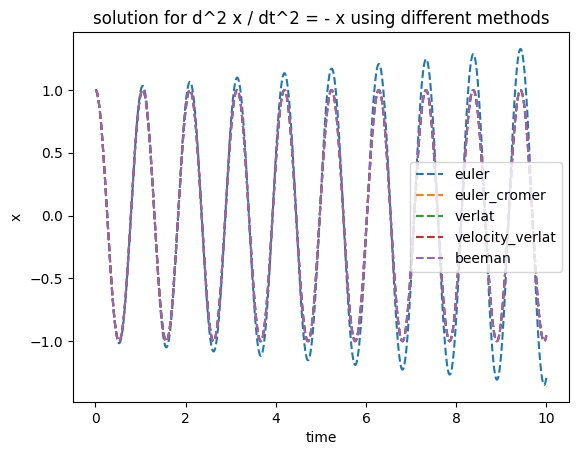
\includegraphics[width=0.8\linewidth]{../p2/ode2_plots.jpg}
		\label{fig:ODEs}
		\caption{plot of the solutions using different integration methods from $0$ to $t = 60$ with time step of $0.01$}
	\end{figure}
	Then, I plotted $\dot{x}$ as a function of $x$ for each method separately. (Fig\ref{fig:energy})
	\begin{figure}[h!]
		\centering
		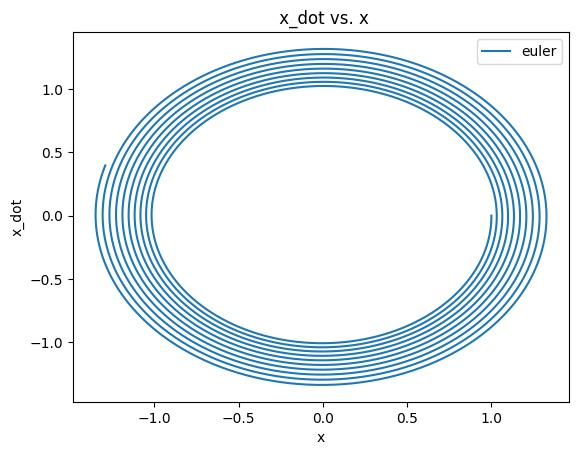
\includegraphics[width=0.45\linewidth]{../p2/euler.jpg}
		\includegraphics[width=0.45\linewidth]{../p2/euler_koomer.jpg}
		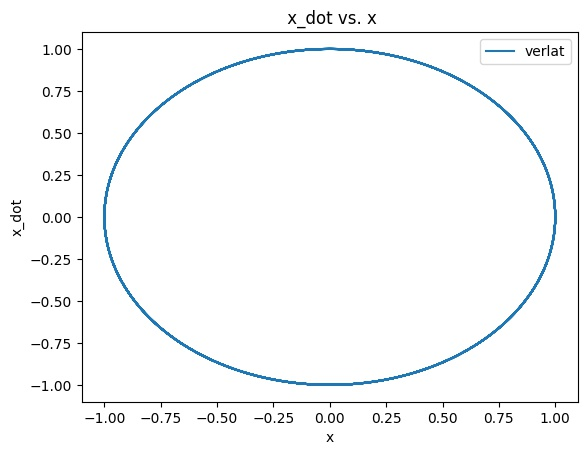
\includegraphics[width=0.45\linewidth]{../p2/verlat.jpg}
		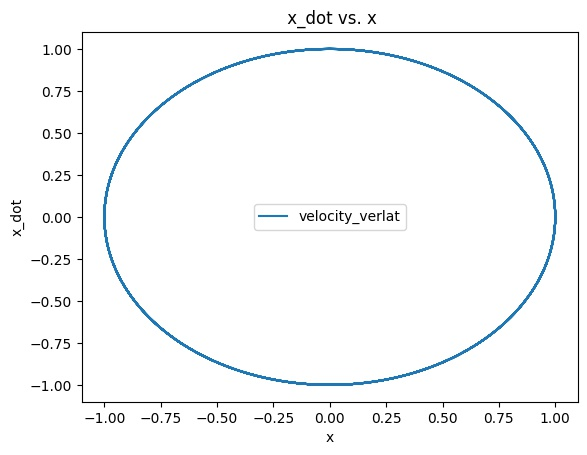
\includegraphics[width=0.45\linewidth]{../p2/velocity_verlat.jpg}
		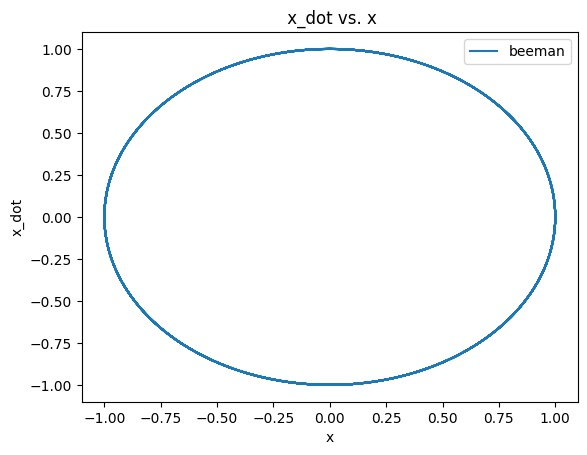
\includegraphics[width=0.45\linewidth]{../p2/beeman.jpg}
		\label{fig:energy}
		\caption{$\dot{x}$ vs. $x$ for different methods.}
	\end{figure}
	
	As can be seen from Fig\ref{fig:energy}, the \emph{verlat}, \emph{velocity verlat}, and \emph{beeman} methods have stability for this
	problem.
	


\end{document}